\nonstopmode
\documentclass[12pt]{report}

\title{Multilayer Perceptrons}
\author{}
\date{\today}

\usepackage[
	top=2cm,
	bottom=2cm,
	left=3cm,
	right=3cm
]{geometry}
\usepackage{amsmath}
\usepackage{amssymb}
\usepackage{amsthm}
\usepackage{listofitems}
\usepackage{amsfonts}
\usepackage{tikz}
\usepackage{pgf}
\usepackage{pgfplots}
\pgfplotsset{compat=1.18}
\usepackage{xcolor}
\usepackage[outline]{contour} % glow around text
\usepackage{hyperref}
\contourlength{1.4pt}


% \usepackage{mathptmx}
% \usepackage{newtxtext, newtxmath}
% \usepackage{stix2}
\usepackage{mlmodern}

\usetikzlibrary{arrows.meta}

% \usetikzlibrary{pgfplots}

\renewcommand{\mod}{\;\text{mod}}
\renewcommand{\qedsymbol}{\blacksquare}

\newcommand{\set}[1]{\left\{ #1 \right\}}
\newcommand{\parens}[1]{\left( #1 \right)}


% Define \bbA ... \bbZ for \mathbb
\newcommand{\bbA}{\mathbb{A}}
\newcommand{\bbB}{\mathbb{B}}
\newcommand{\bbC}{\mathbb{C}}
\newcommand{\bbD}{\mathbb{D}}
\newcommand{\bbE}{\mathbb{E}}
\newcommand{\bbF}{\mathbb{F}}
\newcommand{\bbG}{\mathbb{G}}
\newcommand{\bbH}{\mathbb{H}}
\newcommand{\bbI}{\mathbb{I}}
\newcommand{\bbJ}{\mathbb{J}}
\newcommand{\bbK}{\mathbb{K}}
\newcommand{\bbL}{\mathbb{L}}
\newcommand{\bbM}{\mathbb{M}}
\newcommand{\bbN}{\mathbb{N}}
\newcommand{\bbO}{\mathbb{O}}
\newcommand{\bbP}{\mathbb{P}}
\newcommand{\bbQ}{\mathbb{Q}}
\newcommand{\bbR}{\mathbb{R}}
\newcommand{\bbS}{\mathbb{S}}
\newcommand{\bbT}{\mathbb{T}}
\newcommand{\bbU}{\mathbb{U}}
\newcommand{\bbV}{\mathbb{V}}
\newcommand{\bbW}{\mathbb{W}}
\newcommand{\bbX}{\mathbb{X}}
\newcommand{\bbY}{\mathbb{Y}}
\newcommand{\bbZ}{\mathbb{Z}}


% Define \bfA ... \bfZ for \mathbf
\newcommand{\bfA}{\mathbf{A}}
\newcommand{\bfB}{\mathbf{B}}
\newcommand{\bfC}{\mathbf{C}}
\newcommand{\bfD}{\mathbf{D}}
\newcommand{\bfE}{\mathbf{E}}
\newcommand{\bfF}{\mathbf{F}}
\newcommand{\bfG}{\mathbf{G}}
\newcommand{\bfH}{\mathbf{H}}
\newcommand{\bfI}{\mathbf{I}}
\newcommand{\bfJ}{\mathbf{J}}
\newcommand{\bfK}{\mathbf{K}}
\newcommand{\bfL}{\mathbf{L}}
\newcommand{\bfM}{\mathbf{M}}
\newcommand{\bfN}{\mathbf{N}}
\newcommand{\bfO}{\mathbf{O}}
\newcommand{\bfP}{\mathbf{P}}
\newcommand{\bfQ}{\mathbf{Q}}
\newcommand{\bfR}{\mathbf{R}}
\newcommand{\bfS}{\mathbf{S}}
\newcommand{\bfT}{\mathbf{T}}
\newcommand{\bfU}{\mathbf{U}}
\newcommand{\bfV}{\mathbf{V}}
\newcommand{\bfW}{\mathbf{W}}
\newcommand{\bfX}{\mathbf{X}}
\newcommand{\bfY}{\mathbf{Y}}
\newcommand{\bfZ}{\mathbf{Z}}


% Define \calA ... \calZ for \mathcal
\newcommand{\calA}{\mathcal{A}}
\newcommand{\calB}{\mathcal{B}}
\newcommand{\calC}{\mathcal{C}}
\newcommand{\calD}{\mathcal{D}}
\newcommand{\calE}{\mathcal{E}}
\newcommand{\calF}{\mathcal{F}}
\newcommand{\calG}{\mathcal{G}}
\newcommand{\calH}{\mathcal{H}}
\newcommand{\calI}{\mathcal{I}}
\newcommand{\calJ}{\mathcal{J}}
\newcommand{\calK}{\mathcal{K}}
\newcommand{\calL}{\mathcal{L}}
\newcommand{\calM}{\mathcal{M}}
\newcommand{\calN}{\mathcal{N}}
\newcommand{\calO}{\mathcal{O}}
\newcommand{\calP}{\mathcal{P}}
\newcommand{\calQ}{\mathcal{Q}}
\newcommand{\calR}{\mathcal{R}}
\newcommand{\calS}{\mathcal{S}}
\newcommand{\calT}{\mathcal{T}}
\newcommand{\calU}{\mathcal{U}}
\newcommand{\calV}{\mathcal{V}}
\newcommand{\calW}{\mathcal{W}}
\newcommand{\calX}{\mathcal{X}}
\newcommand{\calY}{\mathcal{Y}}
\newcommand{\calZ}{\mathcal{Z}}

\newcommand{\reffig}[1]{Figure \ref{#1}}

% Math Operators
\DeclareMathOperator{\softmax}{softmax}

% =============================================
% NEURAL NETWORK DRAWING LOGIC 
% =============================================

% COLORS
\colorlet{myred}{red!80!black}
\colorlet{myblue}{blue!80!black}
\colorlet{mygreen}{green!60!black}
\colorlet{myorange}{orange!70!red!60!black}
\colorlet{mydarkred}{red!30!black}
\colorlet{mydarkblue}{blue!40!black}
\colorlet{mydarkgreen}{green!30!black}

% STYLES
\tikzset{
  >=latex, % for default LaTeX arrow head
  node/.style={thick,circle,draw=myblue,minimum size=22,inner sep=0.5,outer sep=0.6},
  node in/.style={node,green!20!black,draw=mygreen!30!black,fill=mygreen!25},
  node hidden/.style={node,blue!20!black,draw=myblue!30!black,fill=myblue!20},
  node convol/.style={node,orange!20!black,draw=myorange!30!black,fill=myorange!20},
  node out/.style={node,red!20!black,draw=myred!30!black,fill=myred!20},
  connect/.style={thick,mydarkblue}, %,line cap=round
  connect arrow/.style={-{Latex[length=4,width=3.5]},thick,mydarkblue,shorten <=0.5,shorten >=1},
  node 1/.style={node in}, % node styles, numbered for easy mapping with \nstyle
  node 2/.style={node hidden},
  node 3/.style={node out}
}
\def\nstyle{int(\lay<\Nnodlen?min(2,\lay):3)} % map layer number onto 1, 2, or 3

\begin{document}

\maketitle

\tableofcontents

\chapter{The Basics of Multilayer Perceptrons}

A \textbf{multilayer perceptron} (otherwise known as a \textit{neural network}) is a set of nodes called \textbf{neurons}, each containing an activation -- a number -- which designates how active that specific neuron is.

This is loosely analogous to how our brains work, where each of our neurons can fire to send an electrical signal which, somewhere down the chain, might move our arm or let us perceive the smell of some food.

The usual image that people associate with neural networks is the following:

\begin{figure}[ht]
	\centering
	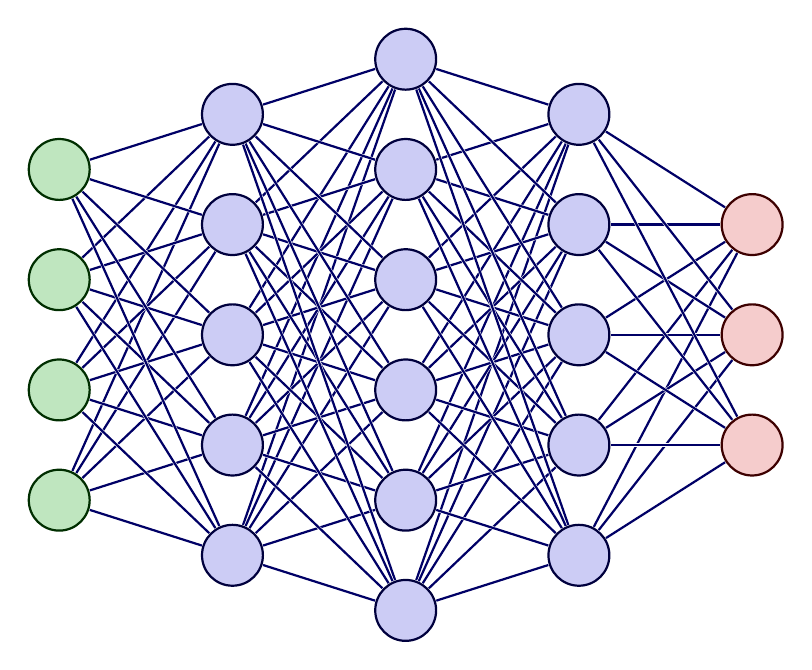
\begin{tikzpicture}[x=2.2cm,y=1.4cm]
		\readlist\Nnod{4,5,6,5,3} % array of number of nodes per layer

		\message{^^J  Layer}
		\foreachitem \N \in \Nnod{
		\def\lay{\Ncnt} % alias of index of current layer
		\pgfmathsetmacro\prev{int(\Ncnt-1)} % number of previous layer
		\message{\lay,}
		\foreach \i [evaluate={\y=\N/2-\i; \x=\lay; \n=\nstyle;}] in {1,...,\N}{ % loop over nodes
			  
				% NODES
				\node[node \n] (N\lay-\i) at (\x,\y) {};

				% CONNECTIONS
				\ifnum\lay>1 % connect to previous layer
					\foreach \j in {1,...,\Nnod[\prev]}{ % loop over nodes in previous layer
						\draw[connect,white,line width=1.2] (N\prev-\j) -- (N\lay-\i);
						\draw[connect] (N\prev-\j) -- (N\lay-\i);
						%\draw[connect] (N\prev-\j.0) -- (N\lay-\i.180); % connect to left
					}
				\fi % else: nothing to connect first layer
			  
			}
		}

		% \node[above=5,align=center,mygreen!60!black] at (N1-1.90) {input\\[-0.2em]layer};
		% \node[above=2,align=center,myblue!60!black] at (N3-1.90) {hidden layers};
		% \node[above=10,align=center,myred!60!black] at (N\Nnodlen-1.90) {output\\[-0.2em]layer};
	\end{tikzpicture}
	\caption{A simple neural network.}
	\label{fig:neural-net-simple}
\end{figure}

\reffig{fig:neural-net-simple} shows the structure of a neural network. At its core, a neural network has an \textbf{input layer} (colored in green), analogous to some sensory input such as our eyes capturing the light around us, an \textbf{output layer} (colored in red), analogous to the output of our vision, which is a colored image of our environment, and then some ``hidden layers,'' which are basically the meat of the network and encode everything about how the inputs and corresponding outputs are related to one another.

\vspace{12pt}

The actual math behind these networks is surprisingly simple. Let's focus in on a single connection for now:

\begin{figure}[ht]
	\centering
	\begin{tikzpicture}
		\def\NI{5}
		\node[node 3] (second) at (2, 0) {$a_1^{(1)}$};
		\foreach \i [evaluate={\y=(\NI + 1) / 2 - \i; \index = int(\i)}] in {1,...,\NI} {
			\node[node 1] (NI-\i) at (-2, \y) {$a_{\index}^{(0)}$}
			\draw[connect] (NI-\i) -- (second) node[midway] {\contour{white}{$w_{1,\index}$}};
		}
	\end{tikzpicture}
	\caption{The activation of two neurons and the weight between them.}
	\label{fig:neuron-activation-example}
\end{figure}

Let's decypher these symbols one-by-one:
\begin{itemize}
	\item ${\color{mydarkgreen} a_n^{(0)}}$: The activations of the nodes within the first layer.
	\item ${\color{mydarkblue} w_{1,n}}$: The \textbf{weights} between each of the connection. Essentially, this encodes how strongly connected the neurons are.
	\item ${\color{mydarkred} a_1^{(1)}}$: The output activation.
\end{itemize}

% \begin{figure}[ht]
% 	\centering
% 	% NEURAL NETWORK activation
% 	% https://www.youtube.com/watch?v=aircAruvnKk&list=PLZHQObOWTQDNU6R1_67000Dx_ZCJB-3pi&index=1
% 	\begin{tikzpicture}[x=2.7cm,y=1.6cm]
% 	  \message{^^JNeural network activation}
% 	  \def\NI{5} % number of nodes in input layers
% 	  \def\NO{4} % number of nodes in output layers
% 	  \def\yshift{0.4} % shift last node for dots
	  
% 	  % INPUT LAYER
% 	  \foreach \i [evaluate={\c=int(\i==\NI); \y=\NI/2-\i-\c*\yshift; \index=(\i<\NI?int(\i):"n");}]
% 	              in {1,...,\NI}{ % loop over nodes
% 	    \node[node in,outer sep=0.6] (NI-\i) at (0,\y) {$a_{\index}^{(0)}$};
% 	  }
	  
% 	  % OUTPUT LAYER
% 	  \foreach \i [evaluate={\c=int(\i==\NO); \y=\NO/2-\i-\c*\yshift; \index=(\i<\NO?int(\i):"m");}]
% 	    in {\NO,...,1}{ % loop over nodes
% 	    \ifnum\i=1 % high-lighted node
% 	      \node[node hidden]
% 	        (NO-\i) at (1,\y) {$a_{\index}^{(1)}$};
% 	      \foreach \j [evaluate={\index=(\j<\NI?int(\j):"n");}] in {1,...,\NI}{ % loop over nodes in previous layer
% 	        \draw[connect,white,line width=1.2] (NI-\j) -- (NO-\i);
% 	        \draw[connect] (NI-\j) -- (NO-\i)
% 	          node[pos=0.50] {\contour{white}{$w_{1,\index}$}};
% 	      }
% 	    \else % other light-colored nodes
% 	      \node[node,blue!20!black!80,draw=myblue!20,fill=myblue!5]
% 	        (NO-\i) at (1,\y) {$a_{\index}^{(1)}$};
% 	      \foreach \j in {1,...,\NI}{ % loop over nodes in previous layer
% 	        %\draw[connect,white,line width=1.2] (NI-\j) -- (NO-\i);
% 	        \draw[connect,myblue!20] (NI-\j) -- (NO-\i);
% 	      }
% 	    \fi
% 	  }
	  
% 	  % DOTS
% 	  \path (NI-\NI) --++ (0,1+\yshift) node[midway,scale=1.2] {$\vdots$};
% 	  \path (NO-\NO) --++ (0,1+\yshift) node[midway,scale=1.2] {$\vdots$};
	  
% 	  % EQUATIONS
% 	  \def\agr#1{{\color{mydarkgreen}a_{#1}^{(0)}}} % green a_i^j
% 	  \node[below=16,right=11,mydarkblue,scale=0.95] at (NO-1)
% 	    {$\begin{aligned} %\underset{\text{bias}}{b_1}
% 	       &= \color{mydarkred}\sigma\left( \color{black}
% 	            w_{1,1}\agr{1} + w_{1,2}\agr{2} + \ldots + w_{1,n}\agr{n} + b_1^{(0)}
% 	          \color{mydarkred}\right)\\
% 	       &= \color{mydarkred}\sigma\left( \color{black}
% 	            \sum_{i=1}^{n} w_{1,i}\agr{i} + b_1^{(0)}
% 	           \color{mydarkred}\right)
% 	     \end{aligned}$};
% 	  \node[right,scale=0.9] at (1.3,-1.3)
% 	    {$\begin{aligned}
% 	      {\color{mydarkblue}
% 	      \begin{pmatrix}
% 	        a_{1}^{(1)} \\[0.3em]
% 	        a_{2}^{(1)} \\
% 	        \vdots \\
% 	        a_{m}^{(1)}
% 	      \end{pmatrix}}
% 	      &=
% 	      \color{mydarkred}\sigma\left[ \color{black}
% 	      \begin{pmatrix}
% 	        w_{1,1} & w_{1,2} & \ldots & w_{1,n} \\
% 	        w_{2,1} & w_{2,2} & \ldots & w_{2,n} \\
% 	        \vdots  & \vdots  & \ddots & \vdots  \\
% 	        w_{m,1} & w_{m,2} & \ldots & w_{m,n}
% 	      \end{pmatrix}
% 	      {\color{mydarkgreen}
% 	      \begin{pmatrix}
% 	        a_{1}^{(0)} \\[0.3em]
% 	        a_{2}^{(0)} \\
% 	        \vdots \\
% 	        a_{n}^{(0)}
% 	      \end{pmatrix}}
% 	      +
% 	      \begin{pmatrix}
% 	        b_{1}^{(0)} \\[0.3em]
% 	        b_{2}^{(0)} \\
% 	        \vdots \\
% 	        b_{m}^{(0)}
% 	      \end{pmatrix}
% 	      \color{mydarkred}\right]\\[0.5em]
% 	      {\color{mydarkblue}\mathbf{a}^{(1)}} % vector (bold)
% 	      &= \color{mydarkred}\sigma\left( \color{black}
% 	           \mathbf{W}^{(0)} {\color{mydarkgreen}\mathbf{a}^{(0)}}+\mathbf{b}^{(0)}
% 	         \color{mydarkred}\right)
% 	    \end{aligned}$};
	  
% 	\end{tikzpicture}
% 	\caption{The calculation for the activation $a_1^{(1)}$.}
% 	\label{fig:neural-net-focus-node}
% \end{figure}

\end{document}